%%%%%%%%%%%%%%%%%%%%%%%%%%%%%%%%%%%%%%%%%%%%%%%%%%
%
% Chapter:  Software Engineering Theory for Team Leaders
%
%%%%%%%%%%%%%%%%%%%%%%%%%%%%%%%%%%%%%%%%%%%%%%%%%%

\label{ch:SETheory}
\chapter{Software Engineering Theory for Team Leaders}

\begin{quote}
``I believe that failure is less frequently attributable to either
insufficiency of means or impatience of labour than to a confused
understanding of the thing actually to be done.'' -- John Ruskin
\end{quote}


TODO:

\begin{itemize}
\item Three Pioneers: Brooks, Lehman, Glass
\item  Beck's Law: ``Maintenance is the normal state'', Extreme Programming Explained, pp. 135.
\begin{itemize}
	\item 60/60 Rule
	\item ``No Silver Bullet'' - Brooks again.
	\item Three historical fallacies (The fallacy of perfect knowledge, the fallacy of the big round ball and the fallacy of perfect execution) from thesis, Ch 2.
\end{itemize}
\item Brook's Law: ``Adding people to a late software project makes it later.''
\item Wood's Law:
\begin{itemize}
	\item Formal: ``A Lehman E-type software system is defined to be in maintenance failure when knowledge of its design and implementation is lost. Avoidance of maintenance failure therefore entails constant actions toward knowledge retention.''
	\item Informal: ``Losing knowledge of a software product causes maintenance failure.''
\end{itemize}
\end{itemize}

\textbf{TODONEXT}: ADD/FIX REFERENCES FROM THESIS.


Software engineering theories as developed both within and outside of academia would seem to have very little bearing upon the average software developer. The daily tools of a developer have certainly benefited from the decades, or even centuries, of mathematical research into logic, the physics, chemistry and electrical engineering used to construct their machinery, the computer science used to develop their operating system, device drivers, major algorithms, and languages, and even the interface design to be found in their application development environments. Software engineering, as a discipline, seems at best to be missing and at worst to be missing the point.

All of that changes when you become a team leader. Suddenly, software engineering theory has a lot to say about how you should pursue your daily tasks, and explains why you should do so.

\section{Three Pioneers: Brooks, Lehman, Glass}

Three computing pioneers attempted to define and collect ``laws'' of software evolution: Fred Brooks, Meir Lehman and Bob Glass. All three began their careers in industry, and all three ended as academics. It is instructive to review them briefly to see how they have stood the test of time, and to note the lessons they present for software team leaders.

Brooks defined four ``inherent properties'' of software based on his experience in the 1960s and 70s at IBM; complexity, conformity, changeability and invisibility \cite{Brooks-1987}. Software is \textit{complex} because programmers continue to define and use new levels of abstraction. This is the reverse procedure from the physical sciences, where practitioners have spent generations by doing the exact opposite. Software becomes more complex as it is forced to \textit{conform} to other systems, some of which are arbitrary (and arbitrarily complex) such as human social systems. Software evolves, it is \textit{changeable} throughout its life cycle. Finally, the geometric abstractions of software are mostly difficult or impossible to visualize. They are, to use Brooks' term, \textit{invisible}.

\textbf{TODO}: Add a label and reference to Appendix A
Lehman was the first to recognize that software evolves during its lifecycle [Lehman 1969]. Lehman's laws were initially based upon IBM's processes, then grew to encompass other sources. Lehman began to formulate his laws as early as 1974, then systematically sought refinements over more than twenty years \cite{Lehman-1997}.

Lehman specifically defined several types of software systems, but his laws only apply to ``evolving'' or E-type systems. The other types are those defined entirely by their specifications or procedures. Such systems are rare indeed. E-type systems are the most common type of software systems because they are those that model, and thus to need to track and respond to, changing real-world situations.

Lehman defined eight laws relating to E-type systems. Arguably the two most important echo Brooks: The Law of Continuing Change notes that a software project evolves continuously (Brooks' changeability) and the Law of Increasing Complexity suggests that a software project becomes less structured, or more complex, with time (Brooks' complexity and conformity). One may also consider Lehman's Law of Declining Quality, which states that a project's quality decreases during its lifecycle unless specific efforts are made to address it, although that would appear to be a consequence of increasing complexity.

Glass collected fifty-five ``facts'' of software engineering through the arduous process of surveying many different types of software development organizations in multiple countries over many years. He summarized his collected facts into four themes: complexity, poor estimation coupled with schedule pressure, a disconnect between software managers and technologists, and the delusion of hype. Glass concluded his multi-decadal study by saying, ``I would suggest that practitioners considering some tool, technique, method or methodology that is at odds with one or more of these facts should beware of serious pitfalls in what they are about to embark on.'' \cite{Glass-2003}, pp 187.

Applicability challenges to both Lehman and Glass were made during the 1990s, as Free/Libre/Open Source software models for development began to become commonplace. Glass even went so far as to state an opinion that Open Source software would not long survive in the market. In spite of this, the established laws of software engineering have continued to hold. Challenges today tend to be minor, and in very particular circumstances. All three models have been shown to hold across many domains, including Open Source development.

Of the three, it is Lehman that has long been recognized as the hallmark of the field. Perhaps the reason for this is simply that Lehman's laws are more detailed than Brooks', but easier to understand than the many facts put forth by Glass. That they all point in the same direction is comforting.

Lehman's laws are presented in more detail in Appendix \ref{app:LehmansLaws}.

One embarks on a career in software management without an understanding of Brooks' inherent properties, Lehman's Laws and Glass's Facts at their peril. The work of software engineering theorists can and does guide good managers toward the most effective management strategies. The remainder of this chapter will demonstrate exactly how this is so.


\section{Problems with the Building Metaphor}

\begin{quotation}
``Software is largely a service industry operating under the persistent but unfounded delusion that it is a manufacturing industry.'' -- Eric Raymond
\end{quotation}

TODO: A bit of history regarding design, development, and project management inherited from the other engineering disciplines.

TODO: Brooks recognized the limits of the building metaphor back in 1958, and wrote about its flaws through the end of his career. In his seminal 1986 essay ``No Silver Bullet'', he stated,

\begin{quotation}
The building metaphor has outlived its usefulness. It is time to change again. If, as I believe, the conceptual structures we construct today are too complicated to be accurately specified in advance, and complex to be built flawlessly, then we must take a radically different approach.
\end{quotation}

The approach that Brooks intended to take was to grow software, rather than build it. He specifically used evolutionary metaphors TODONEXT. Note how this presaged Scrum and Agile development.


\section{What We Mean by ``Maintenance''}

\begin{quote}
``Computer Science is the only discipline
in which we view adding a new wing to a building as being maintenance.'' -- Jim Horning
\end{quote}

TODO: Clean and fix.
Software has long been one of the most complex structures created by humans [Brooks 1987] and often the most expensive portion of engineered systems that include it, as foreseen in the 1970s by Barry Boehm [Boehm 1973]. Software maintenance is, often by far, the largest portion of the software lifecycle in terms of both cost and time [Glass 2003, pp. 115-124]. Software maintenance is thus critically important to the economics of modern engineered systems, from phones to cars, industrial furnaces to spacecraft. Yet, in spite of thirty years of study of the mechanisms and attributes of maintenance activities, there exist a number of significant open problems in the field. Software still becomes unmaintainable with time [Jones 2007] (known formally as ``maintenance failure'' and informally as ``bit-rotting'').

Maintenance failure is exacerbated by the rapid divergence of software systems and information about them. This divergence is typically a consequence of the loss of coupling between software components and system metadata [Van Doren 1997]. Many researchers have mapped the complicated relationships between software components and system metadata such as requirements, metrics and tests [e.g. Han 1994, Rugaber 2000, Welsh 1994a, Welsh 1994b]. In particular, the need for relational navigation of all of these entities has been recognized [Jarrott 2003]. The key to avoiding maintenance failure is maintaining knowledge of both the design and implementation of a software system.


\section{Confronting Challenges in Evolving Software}

Software maintenance has a checkered past.  It has been relatively ignored in favor of tools and techniques for software development.  Thus, a comment on the state of the field in 1983 (``Software maintenance has been almost always neglected'' [Parikh 1983, pp.8]) sounds much like a comment from 2003 (``... the computer science or software engineering curriculum that contains material on software maintenance is rare indeed.'' [Glass 2003, pp. 116]).  Software maintenance is so under-discussed and under-valued that it was possible for at least one author to publish a book on a software development methodology as late as 2000 without once mentioning maintenance. Recognizing that all may not proceed perfectly during initial development, the author of that methodology stated simply that, ``Corrections of errors or added materials are sent to the recipients of the original report with an explanatory letter.'' [Sandq 2000, page 235]  In spite of significant effort by software engineering theorists, such a blithe attitude toward maintenance is not uncommon, especially among consultants and developers able to pass maintenance tasks to others.

The earliest large-scale software systems were naturally reflections of their funding models.  Military and large corporations dominated funding and therefore development and use.  A smaller percentage of software systems developed in 2008 are developed for military and corporate users due to the existence of software products aimed at consumers.  Tools and techniques developed to assist development (such as packaging of code into libraries, use of version control systems, testing and logging systems, integrated development environments and higher-level languages) enabled a broader application of software.  Software was applied to a wide range of small and large business problems and even personal projects throughout the 1990s and 2000s.  By that time, software was no longer solely the purview of governments and large corporations.  Software maintenance became, and remains, everyone's problem.

There are provable costs to maintenance, such as the number of programmers, their equipment and facilities. Interestingly, the history of maintenance cost estimates shows that they have changed little in spite of radical changes in development tools and techniques. Maintenance today accounts for 40-80\% of a software project's total cost, with an average of 60\% [Glass 2003, pp. 115].  Earlier estimates were similar (and probably relied upon by Glass):  Shooman estimated 30-80\% in 1983 [Shooman 1983, pp. 16], in 1988 Yourdon said 50\% [Yourdon 1988, pp. 24], Pressman said 50-70\% [Pressman 1988, pp. 203], and Shere 60-70\% [Shere 1988, pp. 60].  Pressman went on to warn that, ``If your numbers indicate substantially less effort, it is probably an indication that much maintenance work is going unrecognized.'' [Pressman 1988, pp. 203]

Field deployment of software can lead to substantially worse maintenance scenarios, from high cost to loss of material or life.  A widely referenced U.S. Air Force project in 1976 was reported to cost \$75 per instruction to develop but \$4000 per instruction to maintain due to the inaccessibility of the components [Shooman 1983, pp. 484].  Field deployment still causes maintenance failures even though distributed computing techniques and the Internet now allow software to be remotely patched more easily. Field deployment exacerbated resolution of the infamous ``Year 2000 bug'' because many systems using two-digit year date handling routines were embedded in small devices such as handheld instruments and remote sensing kits [Jones 2006].  An extreme modern example is the onboard software update that caused a battery failure in the Mars Global Surveyor spacecraft in 2007 [Dunbar 2007].

Methodologies have been developed to address obvious failures in the management of software.  They have, almost exclusively, focused on development and not on maintenance.  Fred Brooks famously compared system development experiences of the 1970s to California's La Brea Tar Pits, where many dinosaurs struggled, died and became fossilized warnings to others: ``Large and small, massive and wiry, team after team has become entangled in the tar.  No one thing seems to cause the difficulty -- any particular paw can be pulled away.  But the accumulation of simultaneous and interacting factors brings slower and slower motion.'' [Brooks 1995, pp. 4]  Resulting systems were often functional, but also late, expensive and difficult to maintain.  Systematic efforts to find and fix each difficulty led to a series of software creation techniques, initially several forms of structured programming.  One of the goals of structured programming was to create systems that were readily modifiable or, in other words, maintainable [Martin 1985, pp. 4-5].

Unfortunately, structured programming, like other methodologies before and since, failed to address aspects of development that would later become critical for maintenance.  Jackson Structured Development (JSD), for example, started by describing the structure of each input and output data stream, not by performing analysis of a problem to be solved [Jackson 1983, pp. xii].  Most structured design methodologies emphasized the creation of maintainable systems based upon a combination of up-front design and documenting the code [Yourdon 1988, pp. 24-25].  These techniques are now seen as insufficient due to the constantly changing nature of requirements.  Perhaps they were known to be insufficient then, as well.  Yourdon said in the same work, ``Maintenance programming is a serious problem'' and had only experimental restructuring engines to suggest to those in need.  His work presumed that his readers were coding from scratch.

The role of documentation, either external or internal to a program, is primarily to assist maintenance efforts. Early and current researchers [e.g. from Boehm 1981 to Wiegers 2001] believe that documentation is the key to maintaining software systems, and regularly admonished practitioners for failing to keep it up to date.  Practitioners, in their turn, responded with an unwillingness to contribute to an inherently unreliable medium and a stubborn refusal to ignore schedule pressures. Documentation is generally out of date and incomplete at any stage of the software life cycle [Glass 2003, pp. 123]. Updating documentation is often treated as a chore, often not as an important part of a software deliverable. When documentation is created, it is most often created in isolation from the code itself.  Software without adequate documentation is thus created every day, in spite of the continued appearance of new development tools and methodologies. These factors collude to mortgage the future success of a software project and make maintenance progressively harder [Wiegers 2001].

Maintenance of structured code, like its successor object-orientation, was presumed to be easier, partially because the code would be easier to read and partially because programmers were encouraged to document their designs and decisions. Specific guidance was commonly given that in-code documentation was to record solely a developer's intent:  ``How [a] module works is not described.  This is best ascertained by \textit{actually reading the code}.'' (emphasis in original) [Martin 1985, pp. 54-57].  Some methodologies, such as Extreme Programming (XP), eschew guidance regarding comments at all and suggest that individual programmers should decide on a personal ``style'' [Beck 2005, pp. 69].  In spite of this, many managers and programmers have attempted to create commenting styles that described the code and were physically attached to it.  Examples include Brooks' self-documenting PL/1 code [Brooks 1995, pp. 173], Knuth's Literate Programming methodology [Knuth 1992], Larry Wall's Plain Old Documentation (POD), a mechanism for attaching documentation to scripts in the Perl language [Wall 1987], the Java programming language's Javadoc tool [Sun Microsystems 1994] and Dimitri van Heesch's Doxygen source code documentation generator [van Heesch 1997].

Lack of accurate documentation leads maintenance programmers to make changes without fully understanding their potential impact.  Software is known to become less reliable over time as successive enhancements during maintenance are made without a full and complete understanding of their impacts on other parts of the system (known as ``bad fix injection'').  As many as 20\% of defect repairs can result in injections of new defects, with the average amount around 7\% [Jones 1995].  Perhaps that value suggests progress; Brooks said in his 1975 classic, ``Fixing a defect has a substantial (20 to 50 percent) chance of introducing another.'' [Brooks 1995, pp. 242]

Roughly half of all working programmers are now engaged in maintaining existing software and that figure appears to be rising rapidly [Jones 2007].  One may view this trend as a measure of success for the software industry; systems that work are kept, not replaced.  It may be time to view software maintenance not as a problem at all, but as a consequence of the malleability of software-based systems.  Glass, a proponent of this idea, has suggested making maintenance a ``magnet'' for experienced programmers [Glass 2006].  That may be difficult to accomplish. Many of maintenance's woes may be laid at the feet of psychology, not engineering.  \textbf{TODO}: As the Vonnegut quote at the opening of Chapter I nicely summarizes, creative people seem to prefer acts of creation to those of maintenance, and that observation is not limited to software.  Learning to navigate someone else's code, using older languages or techniques and rigorously testing is not as fun or as glamorous as seeing a new feature appear in a GUI or seeing a complicated feature work for the first time.  Indeed, a common euphemism for ``programmer'' is ``developer'', not ``maintainer''.

A software system must be replaced when maintenance fails.  Replacement often requires reverse engineering of the original and modified requirements before a new system may be designed. Reverse engineering becomes necessary because the code and the information about the code have diverged to a degree that the best documentation for the system is the code itself. This is known as a "loss of coupling" between the software components and system metadata [Antoniol 2002].  Such a maintenance failure occurs as a direct result of (a) programmers creating new bugs via ``bad fix injection'', (b) breaking the documentation by failing to keep it up to date, and (c) failing to migrate away from aging or removed system dependencies.

\textbf{TODO}: Tie the fix to the above three problems into the last section, where Wood's Law is discussed. Use methodologies, and other processes, to specifically address these three problems!


\section{Mechanisms of Software Evolution}

Software that is maintained clearly changes, and generally becomes more complex, with time.  It may thus be said to ``evolve'' by the definition of that word.  May software be said to evolve in the sense of a Darwinesque evolutionary algorithm?  Meir Lehman suggested that the changes to IBM's OS/360 operating system resembled an evolutionary process [Lehman 1969] seven years before the biologist Richard Dawkins first proposed (in 1976) that many aspects of culture, including tools such as software programs, evolve in a Darwinesque manner, at least by analogy [Dawkins 1989].  Software programs, however, differ greatly from biological organisms.  An obvious and important difference is that the unit of modularity is not an ``individual'' [Nehaniv 2006].

Tools in general seem to evolve from dissatisfaction with their form (``form follows failure'') [Petroski 2006].  Software's form, as a medium for the creation of tools, seems to follow failure as well [Nehaniv 1997].  Both end users' and developers' dissatisfactions cause software to change [Reitz 2006].  There is, perhaps, a parallel to be drawn with biological evolution, where form follows competitive advantage.

Tight coupling of many software components, present in most systems, is known to inhibit evolvability of those systems [Reitz 2006].  The concept of loose coupling, where a relationship between two entities is made resilient to change by minimizing assumptions about the entities themselves, is a tenant of modern software architectures such as the World Wide Web.  The term ``loose coupling'' and its relationship to architectural resilience was borrowed from organizational studies [Weick 1976]. Similarly, the late binding of entity addressing can further reduce coupling [Fielding 2000].  The concepts of loose coupling and late binding are desired architectural properties for distributed software maintenance.

Their environment impacts biological systems continually, but that impact is limited to phenotype.  Only genetic changes, mutations, can be passed to offspring.  Software is not as fortunate.  It has been suggested that development tools, software documentation and even the state of the software itself impact the evolvability of a software system [Wernick 2006].

Mechanisms of software evolvability thus remain poorly understood.  Our immature understanding of how software systems evolve begs the question of how to avoid maintenance failure in existing systems and systems that will be created using existing techniques.  Theories of software evolution do not yet provide sufficient answers.

\section{Defining Software Maintenance}

The classic life cycle of software (i.e., the one software engineers adopted from our civil, mechanical and electrical brethren) places maintenance at the end of a series of linear development steps [Pressman 1988, pp. 5-7].  That makes sense for a bridge and it makes sense for a car.  It makes sense for computer hardware.  It even makes sense for some types of computer software, such as field deployed embedded systems with stable requirements.  There was much debate in the 1970s and 1980s whether it was appropriate for software in general.  At the heart of the debate was whether the addition of new features should be counted as ``maintenance''.  If a requirement changed, was it ``maintenance'' to change the implementing code?  What if a new requirement was added?  During those decades, at the dawn of software engineering research, software maintenance was variously seen as either a separate activity such redesign activities [e.g. Shooman 1983, pp. 16, 484] or not [e.g. Brooks 1995 pp. 242, Parikh 1983 pp. ix, Yourdon 1988 pp. 24].  The latter view eventually came to dominate, with some researchers expressing frustration with the definition but noting its common usage ([e.g. Martin 1983, pp. 4]).  The single fact that redesign activities are considered part of software maintenance separates software, conceptually and actually, from every other engineering discipline.

Redesign occurs because requirements change constantly.  Changing requirements were seen in the early days of software engineering as an unfortunate, and even avoidable, side effect of poor initial analysis. A study performed in 1976 reported that the top reasons for the high cost of software were ``user demands for enhancements'' and poor documentation [Shooman 1983 pp. 484-5].  If we adopt the perspective championed by Glass, however, we can see that user demands for enhancement are a feature, not a bug.  The total system cost of software may be high, but software allows us to create systems that simply would not be possible without it.  Consider what our systems would look like (and cost!) if they could only use hardware components.  Importantly, enterprises in a capitalist system exist within a competitive environment.  They must either adapt, or perish.  Other consumers of software, such as militaries, also compete.  The software that supports them must do the same.  Requirements are therefore bound to change constantly.

Researchers in the 1980s attempted to apply concepts of more mature engineering disciplines to software.  This thinking by analogy yielded some important insights, but eventually met with failure as the analogy was stretched beyond its limit.  Software, as we have already shown, is not analogous to hardware in terms of maintenance.  The classic production lifecycle was applied to software in spite of its inapplicability.  Pressman, for example, described maintenance as ``the reapplication of each of the preceding activities for existing software'' [Pressman 1988, pp. 6].  Development of software does not stop.  In other words, software development is not constrained by the mere fact of a delivery.  Delivery may, and usually does, occur many times in the course of a product.

Fully 60\% of maintenance activities relate to user-generated enhancements [Glass 2003, pp. 117].  Coupled with the fact that 60\% of software lifecycle costs relate to maintenance we get the so-called 60/60 Rule, one of the few proposed ``laws'' of software maintenance [Glass 2003, pp. 115-118].  The 60/60 Rule is shown in Figure 2-1.  Understanding changes to be made is a major activity during maintenance.  30\% of total maintenance time spent on understanding the existing product. [Glass 2003, pp. 115-124 and Shere 1988, pp. 61].  Martin [Martin 1983, pp.4] found that up to 80\% of maintenance activities relate to changing requirements.

\begin{figure}[htbp]
\begin{center}
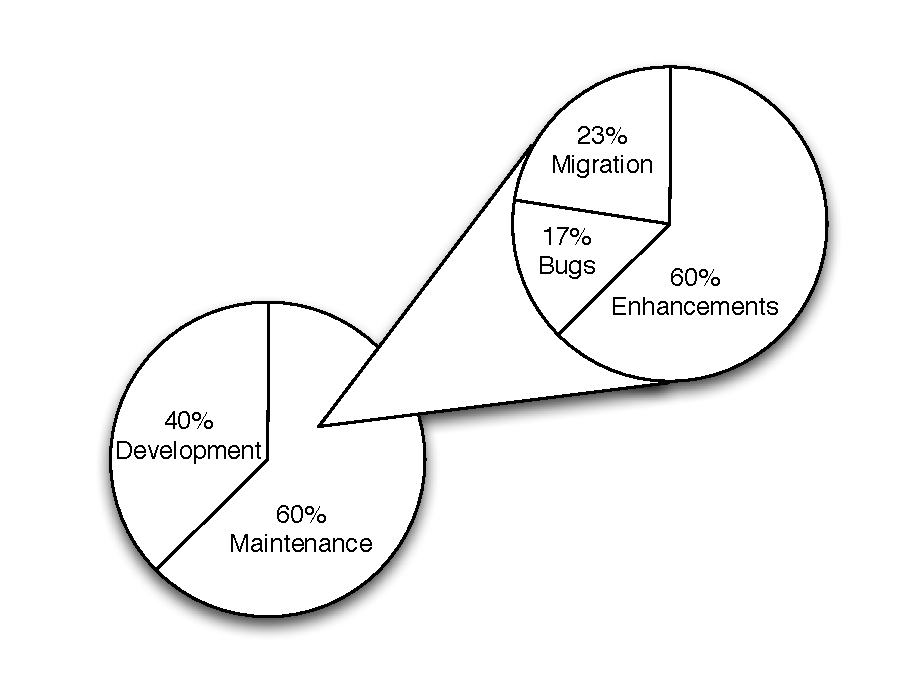
\includegraphics[width=1.00\textwidth]{theory/images/Figure2-1}
\caption{The 60/60 Rule of software maintenance costs.}
\label{fig:2.1}
\end{center}
\end{figure}

The 60/60 Rule should cause us to rethink the focus of software engineering research.  The tendency to address development activities may not yield the most impressive gains.  Boehm's early assertion [Boehm 1981] that proper software engineering discipline can reduce defects by up to 75\% may be true, and became the basis for much work toward development methodologies, but so what?  A good methodology may reduce bugs (17\% of the total maintenance effort), but not address migration or enhancement time or cost at all.

As a software project moves from development activities to maintenance ones, the amount of time spent attempting to understand, trace and redesign (what Glass calls ``undesign'') the code increases.  Testing and debugging time, often related to failures to comprehend a codebase, remain a major factor in spite of the existence of previous tests.  Table \ref{table:2.1} shows the breakdown of developer time spent during development and maintenance.

\begin{table}
    \centering
    \begin{tabular}{| l | c | c |}
    \hline
    \textbf{Task} & \textbf{Development} & \textbf{Maintenance} \\ \hline
    Understanding requirements & 20\% & 15\% \\ \hline
    Design/undesign & 20\% & 30\%  \\ \hline
    Implementing & 20\% & 20\%  \\ \hline
    Testing \& debugging & 40\% & 30\%  \\ \hline
    Documentation & & 5\%  \\ \hline
    \end{tabular}
    \caption[Table caption text]{Typical developer time spent during development and maintenance activities.}
    \label{table:2.1}
\end{table}


Maintainers were originally thought to be spending the bulk of their maintenance time creating enhancements because requirements were poorly captured.  See Figure TODO:2-2. It now seems that maintainers spend the bulk of their time changing requirements specifically because they can [Glass 2006].  Software, as Glass pointed out, is malleable.  Users, managers and investors generally see an economic benefit from modifying an existing system that almost meets their current requirements rather than creating a new one.

\textbf{TODO}: Expand here about the benefits of software: e.g. the number of MSL software updates compared with the number of hardware updates (zero). That just wouldn't be possible without software's malleable (and transmittable) properties.

Judged in that light, Boehm's statement that 20\% of defects account for 80\% of the work and 20\% of the modules account for 80\% of the defects [Selby 2007, pp. 3] would appear to be a benefit.  Poorly designed areas tend to cluster and may be refactored in one place.  New requirements, on the other hand, may or may not cluster, but directly leverage the malleability that is a central property of software.

\begin{figure}[htbp]
\begin{center}
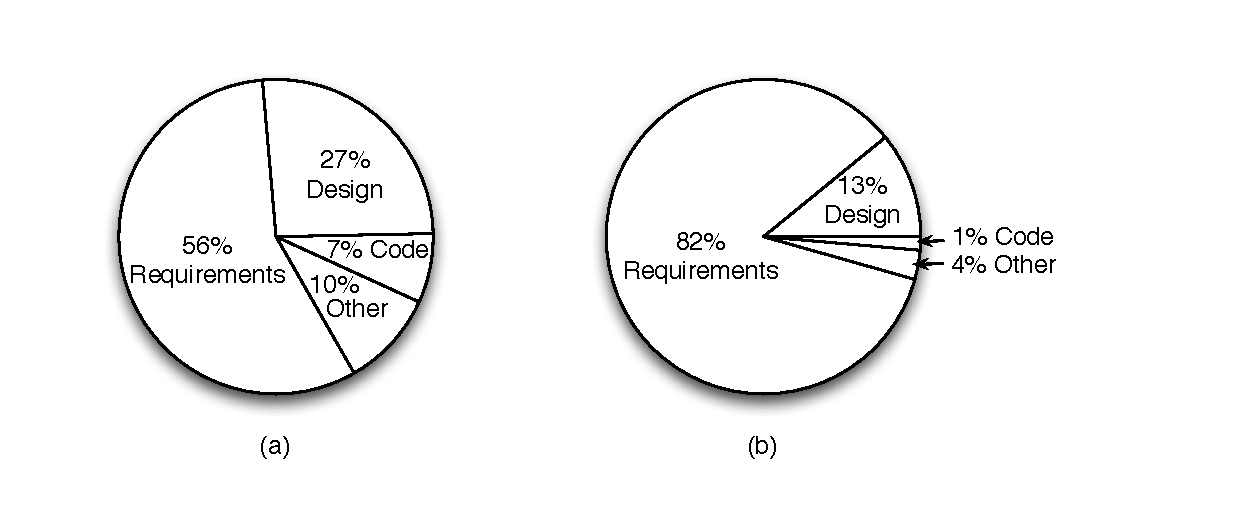
\includegraphics[width=1.00\textwidth]{theory/images/Figure2-2}
\caption{(a) The greatest number of bugs occur in requirements specification and design, (b) The greatest cost is incurred in correcting requirements bugs (After Martin 1983, Figure 12-3).}
\label{fig:2.2}
\end{center}
\end{figure}

Jones [Jones 2007] has refined the definition of software maintenance with a detailed delineation of twenty-three separate forms of modification.  However, he notes that each may be categorized as either defect repair or enhancement.  In my opinion, Jones does not change the definition of maintenance; he details it.

Acknowledging that redesign efforts are part of the software maintenance definition, we can still find obvious differences between creating enhancements and repairing defects.  Defect repairs, be they the result of bad fix injection, poor requirements gathering or failure to correctly implement a feature, do not require changes to the way the software is managed; the original expectation was one of defect-free operation already.  Enhancements, on the other hand, are expected to change the way the software operates, are documented and are tested.  Table \ref{table:2.2} summarizes the key differences.

\begin{table}
    \centering
    \begin{tabular}{| l | c | c |}
    \hline
    & \textbf{Enhancements} & \textbf{Defect Repairs} \\ \hline
    Funding Source & Clients & Developer \\ \hline
    Requirements & Formal & None  \\ \hline
    Specifications & Formal & None  \\ \hline
    Inspections & Formal & None  \\ \hline
    User documentation & Formal & None  \\ \hline
    New function testing & Formal & None  \\ \hline
    Regression testing & Formal & Minimal  \\
    \hline
    \end{tabular}
    \caption[Table caption text]{Typical differences between enhancements and defect repairs.}
    \label{table:2.2}
\end{table}

Clearly, some programmers will perform testing and update documentation (or even specifications and requirements) after repairing a defect, but the practice is all too uncommon.  Table \ref{table:2.2} should not be read as a criticism of programmer practices, but as recognition of trends in current practice.  Thus, the title of the table denotes ``typical'' differences between enhancements and defect repairs.

The Institute of Electrical and Electronic Engineers (IEEE) and the Association for Computing Machinery (ACM) have jointly defined software maintenance as, ``the process of modifying a software system or component after delivery to correct faults, improve performance or other attributes, or adapt to a changed environment'' [IEEE Standard Glossary 1990].  We note that the term ``delivery'' is ambiguous and suggests a classical view of the software lifecycle.  ``Delivery'' in the modern sense can constitute any number of production software releases or updates from conceptualization to retirement of a software product.


\section{Maintenance Failure}

A software product will eventually reach the end of its useful life.  The goal of software maintenance is to delay the end of life as long as possible.  Accordingly, the end of life for a software product is often a state known as ``maintenance failure''.  Maintenance failure eventually occurs in any software product that encodes requirements that remain extant.  Software products whose need is superseded (e.g. a product that calculates wholesale tax following the introduction of a comprehensive goods and services tax) may be removed from service prior to entering maintenance failure.

Maintenance failure may occur for several reasons.  The most common are that a product fails to adapt to changes in environment (such as hardware, operating system or necessary libraries) or it fails to adapt to new requirements.  The latter occurs when new requirements can no longer be added economically. [Brown 1980 pp. 279, Beck 2005 pp. 137]

Early researchers believed the solutions to maintenance failure were straightforward. After analyzing hundreds of software defects in the 1970s, pioneer researcher Barry Boehm said, ``if more time had been spent on validating the design... prior to coding many of the conceptual errors would not have been committed to code.'' [Selby 2007, pp. 1]  Note the connection to Figure TODO:2-2.  Boehm missed the connection from constantly changing requirements to constantly adding value by adapting to changing needs.

Shooman suggested in 1983 that poor documentation is the cause of maintenance failure: ``If the program is to be changed several times over a 10-year period, the documentation is more important than code... Obviously, in any sensible project we want both code and documentation.'' [Shooman 1983, pp. 486] ``It would be wise to pay, say, 10 percent more for the development of reliable software with proper documentation.  This will more than pay for itself in the long run through reduced maintenance and ease of redesign.'' [ibid. pp. 16]  ``The maintenance or modification costs will be strongly related to the quality of the documentation.'' [ibid. pp. 484] Shooman believed that the problems of software maintenance were understood and that the industry was well along the path toward implementing and fielding ``the solution''.  [ibid. pp. 19-20]  Unfortunately, the problems he identified were not solved by a combination of careful development practices and complete documentation.  His hopes for the future included, (a) improved languages and tools, (b) increased use of new development methods and (c) program proofs and automatic programming.  The first two have certainly happened and had an impact on productivity.  The latter has not happened on a large scale.  Although some progress has been recently made in the automated verification of general purpose code, we cannot yet judge how these new techniques will change our abilities to create software [Holzmann 2003].  Increased productivity in development has led to greater, not fewer maintenance challenges.

Yourdon postulated in 1988 that large software projects fail in development due to increasing complexities. ``A project involving up to 100,000 lines of code is sufficiently complex that neither the systems analyst nor the user is likely to have a clear understanding of exactly what the system is supposed to do, and even if there is a clear understanding, the user is likely to change his mind about some of the requirements.'' [Yourdon 1988, pp. 3].  This is the same phenomenon we reviewed earlier when discussing bad fix injection; bad fixes are inserted precisely because the developer does not understand the system.

TODO: Check first reference to Dunbar's Number.
There may be hard limits on our ability as human beings to understand complex systems and those limits are likely to be based in our physiology.  Dunbar's Number [Dunbar 1993] is a (mostly) accepted measure of the number of close interpersonal relationships that may be maintained by a human being.  This limit (roughly 150) is thought to be due to a physiological limitation of the human neocortex.  Human memory also has known limitations.  There are thus limitations to the complexity of a system comprehensible by humans.  One may certainly abstract from the details of a complex system to gain a general understanding or choose to understand a subcomponent in perfect detail.  The perfect understanding of all components coupled with a perfect understanding of the (often conflicting) intents of system users is simply not possible for very large software systems and arguably rare for smaller software systems.  The interpretation of requirements, documentation and code by multiple users, managers, analysts and programmers of a large software project, each according to their own imperfect understanding of what they are attempting to accomplish, merely adds to the complexity of the system.

Software systems and information about them diverge quickly in time, resulting in difficulties understanding and maintaining them.  This divergence is typically a consequence of the loss of coupling between software components and system metadata [Antoniol 2002].   Van Doren discusses an ``Evolution/Replacement Phase, in which the system is approaching or has reached insupportability. The software is no longer maintainable. It has become so 'entropic' or brittle that the cost and/or risk of significant change is too high, and/or the host hardware/software environment is obsolete. Even if none of these is true, the cost of implementing a new requirement is not tolerable because it takes too long under the maintenance environment. It is time to consider reengineering.'' [Van Doren 1997]  It is this type of maintenance failure that we strive most to prevent [Beck 2005, pp. 137].

None of these descriptions of maintenance failure address how we might migrate a software project back from the edge of maintainability; we are more likely to accept the inevitable, abandon the attempt and create a new one.  A primary goal for software team leaders should therefore be to avoid maintenance failure where possible and, where necessary, find means to (slowly, carefully, perhaps even painfully) recover a project's maintainability.  The solution is to lower local entropy and, like any closed system, that means we are required to put work into it.


\section{Three Historical Fallacies}

Much progress was made by the early 1980s in understanding the dynamics of software maintenance.  With a generation of large-scale system implementations behind them and software engineering research well underway, theorists believed that they understood what caused software to become unmaintainable.  Unfortunately, although researchers correctly captured the problems of software maintenance, their solutions were marred by three key fallacies, which we call \textit{The Fallacy of Perfect Knowledge}, \textit{The Fallacy of the Big Round Ball} and \textit{The Fallacy of Perfect Execution}.  As we show below, all three were the direct result of thinking by analogy about the practices of older engineering disciplines.


\subsection{The Fallacy of Perfect Knowledge}

The Fallacy of Perfect Knowledge states that it is possible to capture complete, non-conflicting requirements with sufficient attention to detail.  Requirements, even when agreed upon in detailed up-front design, will change.  It is impossible to know them all in advance.  Requirements gathered from more than one source can also result in inconsistencies.  Requirements may also mean different things to different people.  Differing interpretations may be due to perception, goals or language.  In order to create a general-purpose software maintenance methodology, we must accept and even embrace these ideas.


\subsection{The Fallacy of the Big Round Ball}

The Fallacy of the Big Round Ball states that requirements don't change appreciably after delivery or can be controlled.  Early researchers believed that if requirements could be fully understood before coding began, if the new structured programming techniques were rigidly adhered to, if new systems were documented fully and correctly, there would be no maintenance crisis.  Some academics and practitioners took note of the problem of post-delivery changes to requirements and labeled them evil; static requirements yielded more stable systems.  Some sought to limit a user's right to request changes (e.g., ``Reduce the need for change maintenance by planning for and controlling user enhancements'' -- one of a list of ``solutions to maintenance'' [Martin 1983, pp. 13]).  Unfortunately, such strict controls have the unintended side effect of making a software system less useful to its end users.  Such decisions, often based upon short-term economics, were greatly responsible for the alienation of information technology departments from their user bases in the 1990s and the subsequent development of smaller, often duplicate, software systems within business units during that period.


\subsection{The Fallacy of Perfect Execution}

The Fallacy of Perfect Execution states that it is possible to create flawless code with sufficient attention to detail.  We need to admit that arbitrary logic is hard to verify in the general case, and hard or impossible to fully test.  Drawing an analogy to the bricks and beams used in other construction-related activities, a researcher recently suggested that software is hard to verify because ``there are no good, predictable building blocks.  The elements out of which programs are constructed, statements, procedures, or objects cannot be composed in a predictable fashion'' [Dickerson 2006].  It is also hard to trace programmer intent, especially when requirements change or are inconsistently documented. Bugs will remain part of every software product shipped.

Admitting these three fallacies is tantamount to changing the way we think about the state of software at the end of development.  We can come to see delivered software as buggy, likely to change and with inaccurate documentation.  That insight, simple though it may be, encourages us to approach maintenance differently.  It encourages us to develop tools and techniques to incrementally refactor software implementations, requirements and documentation.


\section{Emerging Problems and Approaches}

Software currently in production was created using a great variety of techniques and procedures.  The software industry continues to struggle with this legacy and is expected to do so for the foreseeable future.  We therefore require a way to record information captured about these programs as they are maintained.  Failure to do that in a systematic manner leaves us where we are now; at the mercy of the memory of individual programmers assigned to a project.

\textbf:{TODO}: Look up relative amounts of procedural, functional, and OO code in production, and quote percentages.

The size of modern projects is increasing dramatically.  In 1988, Yourdon called 10M LOC ``utterly absurd'' [Yourdon 1988, pp. 2], but 2007 saw the Eclipse Foundation release its Europa coordinated project release with seventeen million source lines of code [http://www.linuxdevices.com/news/NS9334092346.html].  Similarly, an official Microsoft blog reported in 2006 that the company's popular Office suite for Macintosh computers measured thirty million source lines of code [http://blogs.msdn.com/macmojo/archive/2006/11/03/it-s-all-in-the-numbers.aspx].  The size of the maintenance domain is clearly increasing.

The key to maintaining complex software systems is to understand them. Victor Basili has said, ``Most software systems are complex, and modification requires a deep understanding of the functional and non-functional requirements, the mapping of functions to system components, and the interaction of components.'' [Basili 1982]  Many researchers have mapped the complicated relationships between domain knowledge, program components and system metadata such as requirements, metrics and tests [e.g. Rugaber 2000, Welsh 1994a].  Some have presaged this thesis in their interpretation of software development as a document-oriented process, and have recognized the importance of inter- and intra-document relationships in supporting traceability from requirements to implementation details [Han 1994, Welsh 1994b].

Research has variously focused on the relationship of program components [Wilde 1990], and the recovery of requirements traceability from source code [Coyle 2002, Antoniol 2002]. Unfortunately, the first is insufficient and the second, in its many forms, is ``not a trivial process'' [Han 1994].  We still require a way to capture and maintain our understanding of a code base that is broadly applicable.

The way we view software for maintenance, as a series of functions to be repaired and added to, is flawed for historical reasons.  The traditional view of a computer was a machine to be commanded via a series of instructions, those instructions being collected into functions.  The functions were collected into a hierarchy (a program), which led naturally to the concept of development structured around functions. [Jackson 1983, pp. 3-4].  We know today that many programs are not hierarchical, such as those designed with grid, object-oriented, message-oriented and resource-oriented architectures.  These more modern logical abstractions for describing computer programs are more Web-like.

\textbf{TODO}: Investigate ``Some problems of hierarchical thinking are investigated in Chapter III.'' Worth adding material here??

Software maintenance and software development, those two states of any software project, need to viewed as the continuum that they are.  Some people are already thinking this way.  So-called Agile methodologies are claimed to be in a constant state of maintenance.  Beck, one of the architects of Extreme Programming, put it this way:  ``Maintenance is really the normal state of an XP project.  You have to simultaneously produce new functionality, keep the existing system running, incorporate new people into the team, and bid farewell to members who move on.'' [Beck 2005, pp. 135-6]  Glass' view of maintenance as a positive outcome of successful projects fits nicely with Beck's model.

\textbf{TODO}: Add a callout box with ``Beck's Law'' here?

Karl Wiegers has gathered a series of principles for approaching requirements maintenance on existing systems [Wiegers 2001].  His collection importantly addresses not only broken code, but also the lack of correct documentation and understanding (of both code and requirements) so common in systems maintained over many years.  He suggests retaining the older documentation, even though it is knowingly out of date, and slowly bringing it to relevancy as one addresses each section of code.  This is a form of documentation refactorization.

A few researchers have attempted to combine the formal methods of software engineering with formal descriptions enabled by Semantic Web technologies (e.g. [Goth 2007]).  Tetlow, for example, claims that some of the benefits of formal methods have not been widely fielded because they are ``too abstract for the average developer''.   The benefit to Semantic Web techniques is that they are unreservedly formal, and yet may be used by developers ``in an exceptionally informal way'' [ibid.].  The W3C has drafted two documents to date dealing with ``Semantic Web-enabled software engineering''; a primer for developers of object-oriented software [Knublauch 2006] and another describing the use of formal ontologies for the description of software systems [Tetlow 2006]. 

\textbf{TODO}: INSERT REFERENCE TO MY OWN THESIS RESEARCH HERE, AND BEST-PAPER FROM IEEE. Note that ``This thesis builds upon Wieger's idea in Chapter VI but extend it in accordance with the metadata best practices for virtual information resources described in Chapter IV.'' and ``This thesis builds on some of the ideas of Semantic Web-enabled software engineering in Chapters VI and VII.''


\textbf{TODONEXT}: Wood's Law, and implications for software team leaders.
\section{Directions for Team Leaders}

A software project dies when it cannot recover from ``maintenance failure'', so focusing effort on maintenance activities that prolong the life of a project makes the most economic sense.

I might modestly call this Wood's Law:

\begin{itemize}
	\item Formal: ``A Lehman E-type software system is defined to be in maintenance failure when knowledge of its design and implementation is lost. Avoidance of maintenance failure therefore entails constant actions toward knowledge retention or knowledge re-acquisition.''
	\item Informal: ``Maintenance failure is caused by the loss of knowledge of a software product.''
\end{itemize}

\vspace{20pt}
\setlength{\fboxsep}{10pt}%
\shadowbox{
\begin{minipage}{11cm}
       \begin{center}
       \textbf{Wood's Law}\\
Maintenance failure is caused by the\\
loss of knowledge of a software product.
       \end{center}
       \end{minipage}
}

\textbf{TODO:} NOTE the lesson for team leaders in a callout box: Optimize for the activities you are mostly doing, not the ones with comparatively little value (such as creating perfect code).

\section{The Dark Art of Estimation}

\textbf{TODO:} Place in relation to old methodologies and their downfall. NOTE the ways that newer methodologies seek to estimate, not exactly schedule like the the old ones.



% If the chapter ends in an odd page, you may want to skip having the page
%  number in the empty page
\newpage
\thispagestyle{empty}
